\chapter{Hadron Therapy}

\section{Introduction}
The National Cancer Institute define a tumor\cite{tumor} as “an abnormal mass of tissue that results when cells divide more than they should or do not die when they should.”
In a healthy body, cells grow, divide, and replace each other in the body. As new cells form, the old ones die. When a person has cancer, new cells form when the body does not need them. If there are too many new cells, a group of cells, or tumor, can develop.
A tumor develops when cells reproduce too quickly. Tumors can vary in size from a tiny nodule to a large mass, depending on the type, and they can appear almost anywhere on the body.
There are three main types of tumor:
\begin{itemize}
\item \textbf{Benign}: These are not cancerous. They either cannot spread or grow, or they do so very slowly. If a doctor removes them, they do not generally return.
\item \textbf{Premalignant}: In these tumors, the cells are not yet cancerous, but they have the potential to become malignant.
\item \textbf{Malignant}: Malignant tumors are cancerous. The cells can grow and spread to other parts of the body.
\end{itemize}
Radiation therapy is the medical use of ionizing radiation to treat cancer. In conventional radiation therapy, beams of X rays (high energy photons) are produced by accelerated electrons and then delivered to the patient to destroy tumour cells. Using crossing beams from many angles, radiation oncologists irradiate the tumour target while trying to spare the surrounding normal tissues. Inevitably some radiation dose is always deposited in the healthy tissues.
When the irradiating beams are made of charged particles (protons and other ions, such as carbon), radiation therapy is called hadron therapy\cite{radiationtherapy}. The strength of hadron therapy lies in the unique physical and radiobiological properties of these particles; they can penetrate the tissues with little diffusion and deposit the maximum energy just before stopping. This allows a precise definition of the specific region to be irradiated. The peaked shape of the hadron energy deposition is called Bragg peak and has become the symbol of hadron therapy. With the use of hadrons the tumour can be irradiated while the damage to healthy tissues is less than with X-rays.

\section{Interaction between matter and charged particles}
Charged particles with mass greater than the one of the electron lose energy in matter through ionization.
A classic calculation for the energy lost in ionization can be done taking into account two assumptions:
\begin{itemize}
	\item the speed of the atomic electron is negligible compared to the one of the incident particle;
	\item the mass of the incident particle is big in relation to the target mass. This means that the incident particle for each single hit receives a small amount of momentum and thus the direction of flight does not changes.  
\end{itemize}
\noindent This hypothesis is valid keeping into consideration that the mass of the electron is 0.51 MeV, a muon has mass 105.6 MeV, for a proton it is 938.2 MeV and for a carbon ion ${}^{12}$C it is 11177.9 MeV.
\newline
The classic calculation results in the Bethe-Block formula in equation \ref{eq:bethe} that describes the average energy loss in the target for unit of length, also called stopping power.
\begin{equation}\label{eq:bethe}
	-\dfrac{\mathrm dE}{\mathrm dx} = 2 \pi N_{a} r_{e}^{2} m_{e} c^{2} \rho \dfrac{Z}{A}  \dfrac{z^{2}}{\beta^{2}}\left[\ln\left(\dfrac{2m_{e} \gamma ^{2} v^{2} W_{max}}{W^{2}}\right) - 2\beta^{2} - \delta 2\frac{C}{Z}\right]
\end{equation}
\noindent In equation \ref{eq:bethe}:
\begin{itemize}
	\item $N_a$: is the Avogadro number;
	\item $r_e$: is the classical radius of the electron;
	\item $m_e$: is the mass of the electron;
	\item $\rho$: target density;
	\item $Z $: target atomic number;
	\item $A $: target atomic mass;
	\item $W $: target average ionization energy;
	\item $z $: incident particle charge;
	\item $W_{max} $: maximum energy transferred in a collision; 
	\item $\delta $: polarization parameter in target
	\item $c/z $: core electrons shielding parameter 
	\item $\beta = v/c $
\end{itemize}
\noindent The stopping power depends by the target mass, atomic number, density and average ionization energy (A, Z, $\rho$, W). To overcome and eliminate this dependence it was defined the massic stopping power in equation \ref{eq:stoppingpower} that is measured in MeV/(g cm${}^2$)
\begin{equation}\label{eq:stoppingpower}
	\delta = - \frac{1}{\rho} \frac{dE}{dx}
\end{equation}
\noindent In figure it can be seen the trend of the massic stopping power of a $\mu^+$ passing through a copper layer.
\begin{figure}[H]
	\centering
	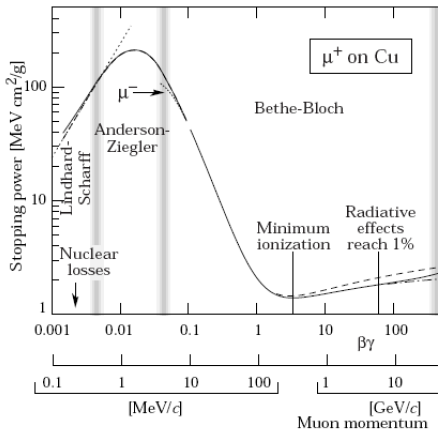
\includegraphics[width=0.7\linewidth]{IMG/ch1/MassicStoppingPower}
	\caption{Massic Stopping power in function of the $\mu^+$ momentum passing through a copper layer}
	\label{fig:massicstoppingpower}
\end{figure}
\noindent In the trend of the stopping power in function of the momentum can be noted a de-growth for low momentum values that is due to the term $\frac{1}{\beta^2}$ in equation \ref{eq:bethe}; the stopping power decreases until it reaches a minimum, and then slowly grows back.
\newline
The average path (range) of a charged particle can be calculated by integrating the stopping power along the "walk".
\begin{equation}\label{eq:range}
	R=\int_{E_i}^{0} \frac{1}{\frac{dE}{dx}}dx
\end{equation}
\noindent The range depends approximately on the A / Z ratio of the material and grows approximately with the square of the initial kinetic energy of the charged particle. The accrual
of energy loss increases as the kinetic energy of the particle decreases with the depth of penetration, with a rapid ascent at the end of the path. The density of ionization of the charged particles along their path in the medium is therefore
characterized by a plateau followed by a pronounced maximum towards the end of range, called Bragg peak, which is located at an energy-dependent depth initial kinetics of the incident particle, as shown in \textbf{Figure 1.2}
If more particles are considered then it should be kept in mind
the statistical fluctuations on the collisions of the particles and on the energy transferred for each collision: these fluctuations are well described by the Landau distribution
\textbf{[2]}, generate uncertainty about the distance reached by the particles ("straggling"). Beyond all these considerations we must not neglect the possible interactions with the nuclear components of the matter crossed. One effect is enlargement
lateral of the beam due to the interaction with the Coulomb fields of the nuclei that it is inversely proportional to the mass of the incident particle. The second effect it is due to the fragmentation of the primary bundle and/or of the nuclei of the material passed through due to nuclear interactions. The fragmentation cross section becomes relevant for ions heavier than the proton, such as carbon ions or heavier, and causes a decrease in the number of particles incident along the path
and the development of secondary fragments. The fragments produced deposit theirs energy deeper than the Bragg peak giving rise to a queue in the distribution.
\begin{figure}[H]
	\centering
	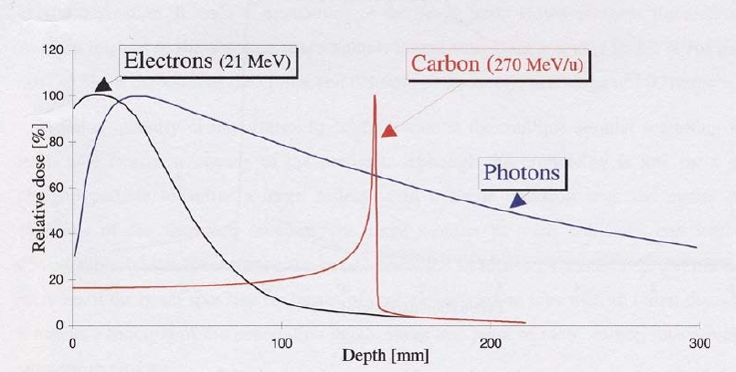
\includegraphics[width=0.7\linewidth]{IMG/ch1/BraggPeak}
	\caption{Dose profile for a 21MeV electron, 270MeV/u carbon ion and photon beam}
	\label{fig:braggpeak}
\end{figure}  

%\begin{equation}\label{eq:bethe2}
%	W_{max} = \dfrac{2m_{e} c^{2} \eta^{2}}{1+2s \sqrt{1+\eta^{2}} + s^{2}};\qquad s=m_{e}/M;\eta=\beta\gamma.
%\end{equation}


\section{Effects of radiations on biological systems}


\section{Dose distribution systems in hadron therapy}

\subsection{Passive dose distribution systems}

\subsection{Active dose distribution systems}

\subsection{Treatment Planning System}

\section{Beam monitoring}

\subsection{Silicon detectors}